\section{Thiết kế hệ thống và Công nghệ}
\sloppy

\subsection{Tổng quan kiến trúc hệ thống}

Hệ thống Smart House được triển khai theo mô hình web application kết hợp IoT gateway. Frontend React/Vite cung cấp giao diện sử dụng, backend Spring Boot xử lý API và nghiệp vụ, PostgreSQL lưu dữ liệu, RabbitMQ phục vụ luồng thông điệp người dùng, còn gateway Python kết nối thiết bị/simulator với backend và dịch vụ camera YOLO.

\begin{figure}[htbp]
    \centering
    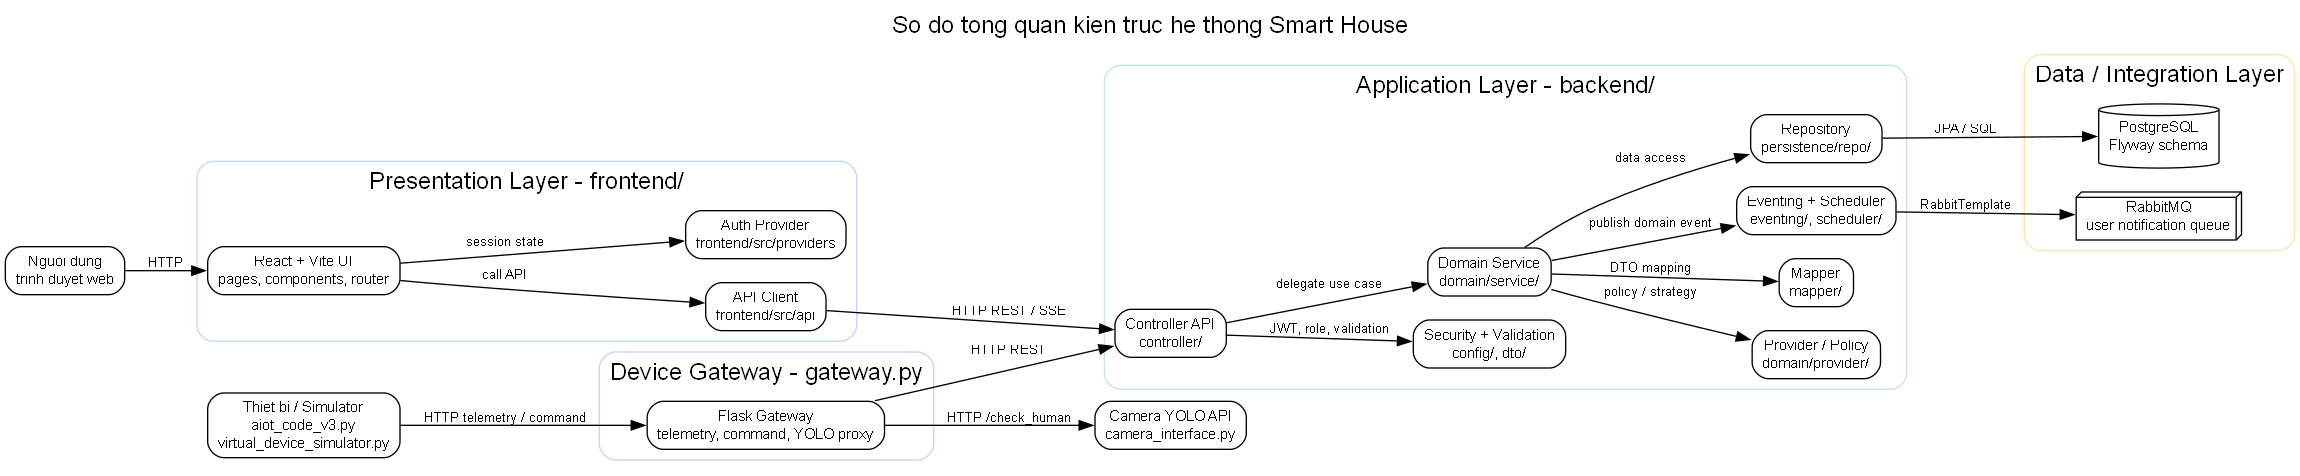
\includegraphics[width=\linewidth,height=0.78\textheight,keepaspectratio]{Images/architecture_overview.png}
    \caption{Sơ đồ tổng quan kiến trúc hệ thống}
    \label{fig:architecture-overview}
\end{figure}

\textbf{Các khối chính trong kiến trúc:}
\begin{itemize}
    \item \textbf{Presentation layer:} nằm trong \texttt{frontend/src}, gồm router, pages, components, provider và API client. Tầng này hiển thị dữ liệu, nhận thao tác người dùng và gọi backend bằng HTTP REST hoặc SSE.
    \item \textbf{Application/API layer:} nằm trong \texttt{backend/src/main/java/com/java/controller}, nhận request, kiểm tra dữ liệu đầu vào và trả response chuẩn qua \texttt{ApiResponse}.
    \item \textbf{Business/service layer:} nằm trong \texttt{domain/service} và \texttt{domain/provider}, xử lý điều khiển thiết bị, telemetry, cấu hình, cảnh báo, lịch, audit, xác thực và tự động hóa.
    \item \textbf{Data access layer:} nằm trong \texttt{persistence/entity} và \texttt{persistence/repo}, ánh xạ JPA entity và truy cập PostgreSQL thông qua repository.
    \item \textbf{Integration layer:} gồm \texttt{gateway.py}, \texttt{camera\_interface.py}, \texttt{adapter}, \texttt{eventing}, \texttt{scheduler} và RabbitMQ.
\end{itemize}

\textbf{Cách giao tiếp giữa các thành phần:}
\begin{itemize}
    \item Trình duyệt người dùng truy cập frontend tại cổng \texttt{5173} khi chạy bằng Docker Compose.
    \item Frontend gọi backend qua \texttt{VITE\_API\_BASE\_URL}; giá trị mặc định trong \texttt{apiClient.js} là \texttt{http://localhost:8080}.
    \item Backend kết nối PostgreSQL bằng JDBC thông qua các biến \texttt{DB\_URL}, \texttt{DB\_USERNAME}, \texttt{DB\_PASSWORD}.
    \item Thiết bị hoặc simulator gửi telemetry tới gateway; gateway chuyển tiếp đến endpoint \texttt{/api/device-telemetry}.
    \item Thiết bị lấy lệnh điều khiển qua endpoint \texttt{/api/v1/device/\{deviceKey\}/commands/next} và xác nhận bằng \texttt{/commands/ack}.
    \item Dashboard nhận realtime event qua SSE của \texttt{DashboardController}.
\end{itemize}

\subsection{Mô hình hóa hệ thống}

\textbf{Sơ đồ use case tổng quan:} Bốn biểu đồ use case trong phần yêu cầu chức năng mô tả các nhóm nghiệp vụ chính của hệ thống, gồm đăng nhập và phân quyền, cấu hình tự động hóa, giám sát telemetry, điều khiển thiết bị, cảnh báo và truy vết hoạt động.

\textbf{Biểu đồ thành phần:}

\textit{Hướng dẫn đọc sơ đồ:} Các biểu đồ thành phần thể hiện cách các khối chức năng phối hợp trong hệ thống Smart Home. Component biểu diễn một khối chức năng của hệ thống; provided interface thể hiện năng lực mà component cung cấp; required interface thể hiện năng lực mà component cần từ component khác; port là điểm giao tiếp của component; đường nối thể hiện quan hệ phụ thuộc hoặc giao tiếp giữa các khối.

\begin{figure}[htbp]
    \centering
    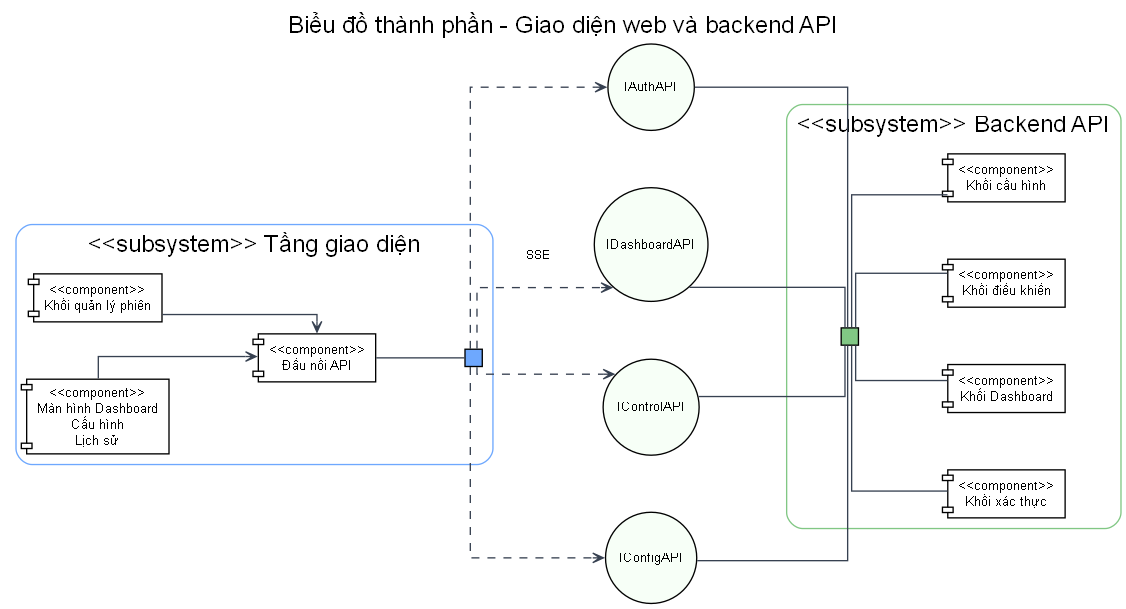
\includegraphics[width=\linewidth,height=0.70\textheight,keepaspectratio]{Images/component_frontend_api.png}
    \caption{Biểu đồ thành phần cho giao diện web và backend API}
    \label{fig:component-frontend-api}
\end{figure}

Biểu đồ thành phần giao diện web và backend API mô tả ranh giới giao tiếp giữa tầng giao diện và các năng lực phía máy chủ. Tầng giao diện tiếp nhận thao tác của người dùng, quản lý phiên đăng nhập và gửi yêu cầu đến các khối xác thực, Dashboard, điều khiển thiết bị và cấu hình tự động hóa.

\begin{figure}[htbp]
    \centering
    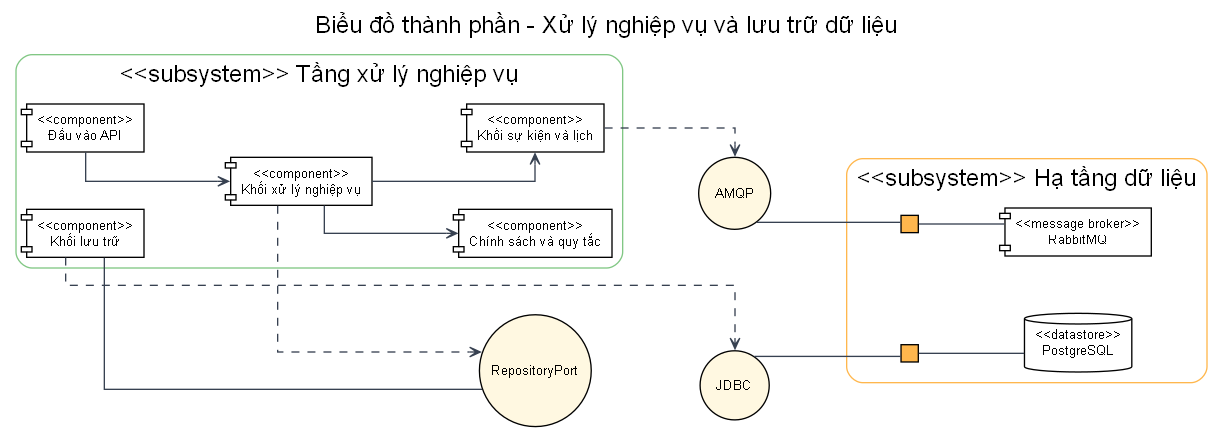
\includegraphics[width=\linewidth,height=0.70\textheight,keepaspectratio]{Images/component_backend_data.png}
    \caption{Biểu đồ thành phần cho tầng xử lý nghiệp vụ và lưu trữ dữ liệu}
    \label{fig:component-backend-data}
\end{figure}

Biểu đồ thành phần tầng xử lý nghiệp vụ và lưu trữ dữ liệu mô tả các khối đảm nhận kiểm tra yêu cầu, áp dụng quy tắc nghiệp vụ, lưu trữ trạng thái hệ thống và phát sinh sự kiện. PostgreSQL lưu dữ liệu bền vững, còn RabbitMQ hỗ trợ các thông điệp bất đồng bộ trong các luồng cần tách rời thời điểm xử lý.

\begin{figure}[htbp]
    \centering
    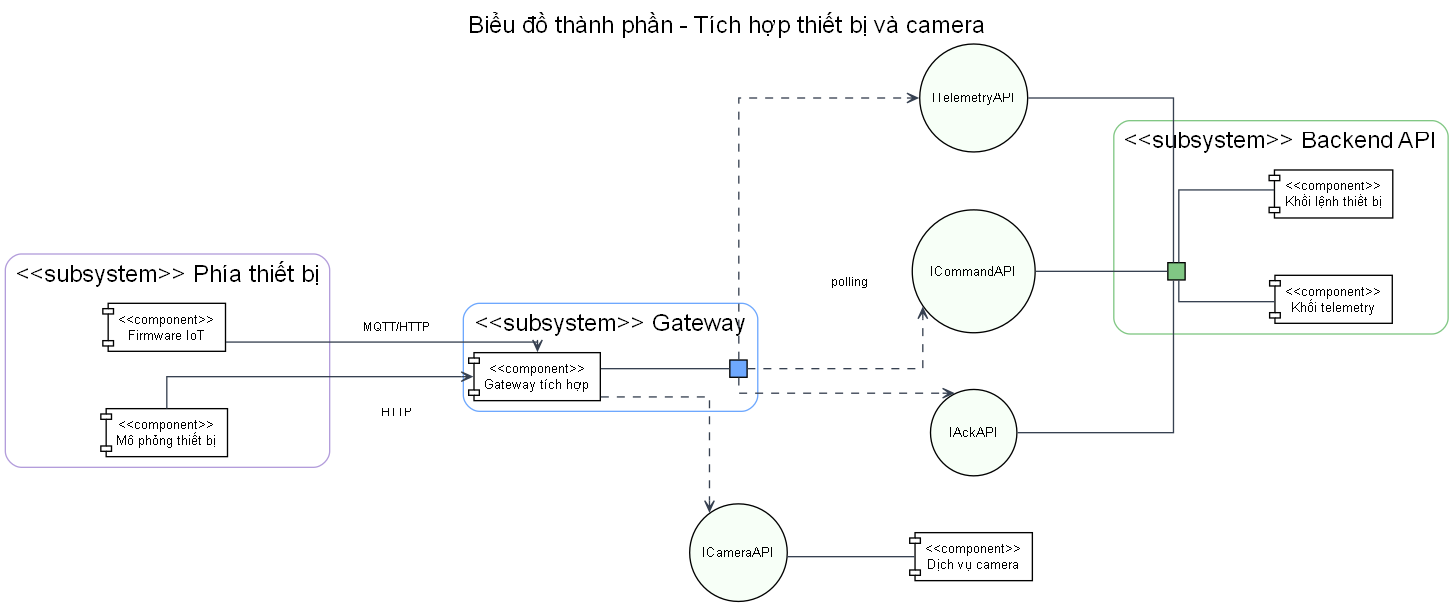
\includegraphics[width=\linewidth,height=0.70\textheight,keepaspectratio]{Images/component_device_integration.png}
    \caption{Biểu đồ thành phần cho tích hợp thiết bị và camera}
    \label{fig:component-device-integration}
\end{figure}

Biểu đồ thành phần tích hợp thiết bị và camera thể hiện gateway là điểm trung gian giữa thiết bị, mô phỏng thiết bị, backend API và dịch vụ camera. Khối này chuyển dữ liệu telemetry, nhận lệnh điều khiển, gửi xác nhận thực thi và gọi dịch vụ nhận diện khi cần thông tin từ camera.

\textbf{Biểu đồ hoạt động cho luồng đăng nhập:}
\begin{figure}[htbp]
    \centering
    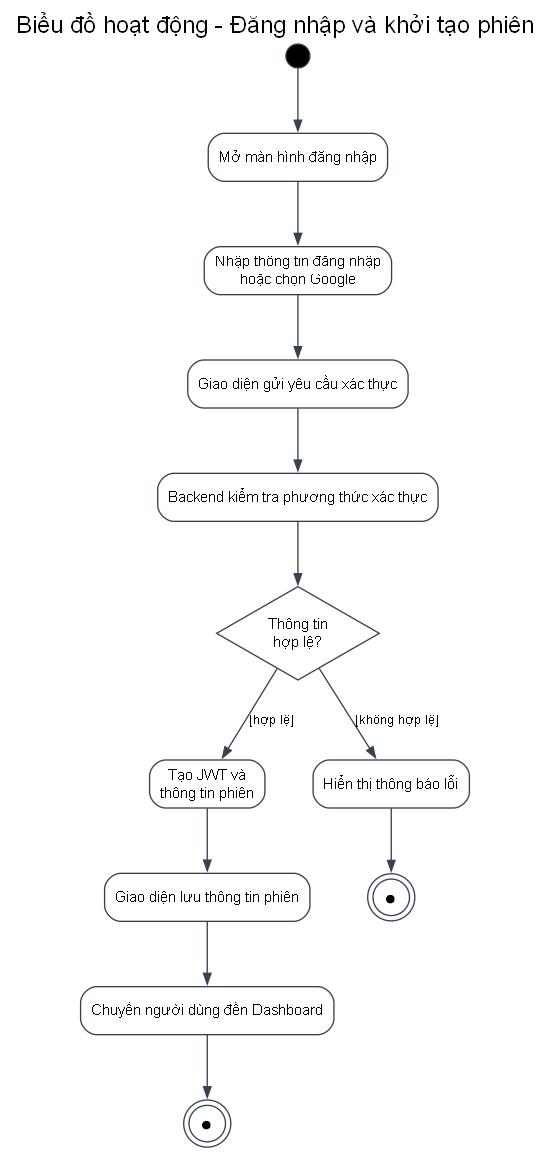
\includegraphics[width=\linewidth,height=0.78\textheight,keepaspectratio]{Images/activity_login.png}
    \caption{Biểu đồ hoạt động cho luồng đăng nhập và khởi tạo phiên}
    \label{fig:activity-login}
\end{figure}

Biểu đồ hoạt động cho luồng đăng nhập mô tả quá trình người dùng mở màn hình đăng nhập, nhập thông tin hoặc chọn Google, sau đó giao diện web gửi yêu cầu xác thực đến backend. Nếu thông tin không hợp lệ, hệ thống hiển thị thông báo lỗi và kết thúc luồng thất bại. Nếu hợp lệ, backend tạo JWT và thông tin phiên, giao diện lưu phiên và chuyển người dùng đến Dashboard.

\textbf{Biểu đồ hoạt động cho luồng telemetry và tự động hóa:}
\begin{figure}[htbp]
    \centering
    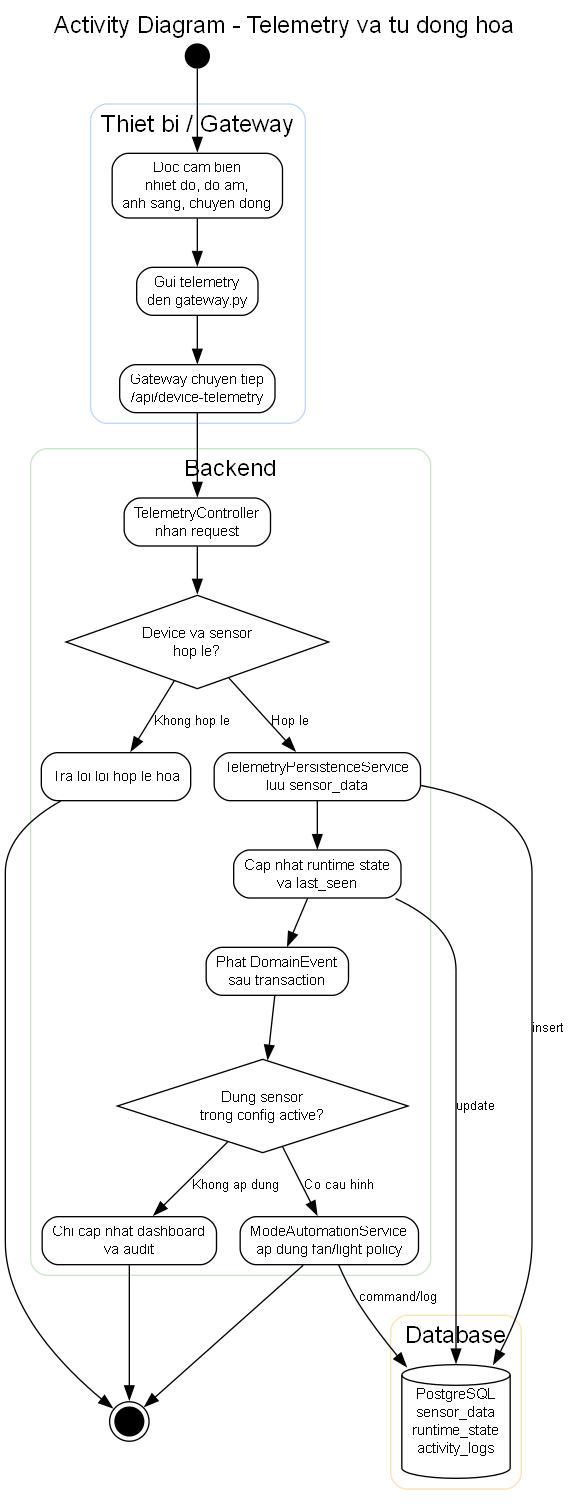
\includegraphics[width=\linewidth,height=0.78\textheight,keepaspectratio]{Images/activity_telemetry_automation.png}
    \caption{Biểu đồ hoạt động cho luồng telemetry và tự động hóa}
    \label{fig:activity-telemetry}
\end{figure}

Luồng telemetry bắt đầu khi thiết bị hoặc bộ mô phỏng gửi dữ liệu cảm biến về hệ thống. Backend kiểm tra tính hợp lệ của thiết bị và dữ liệu, ghi nhận dữ liệu cảm biến, cập nhật trạng thái thiết bị, phát sự kiện nội bộ và đánh giá các quy tắc tự động hóa đang áp dụng cho ngôi nhà.

\textbf{Biểu đồ lớp tổng quan:}
\begin{figure}[htbp]
    \centering
    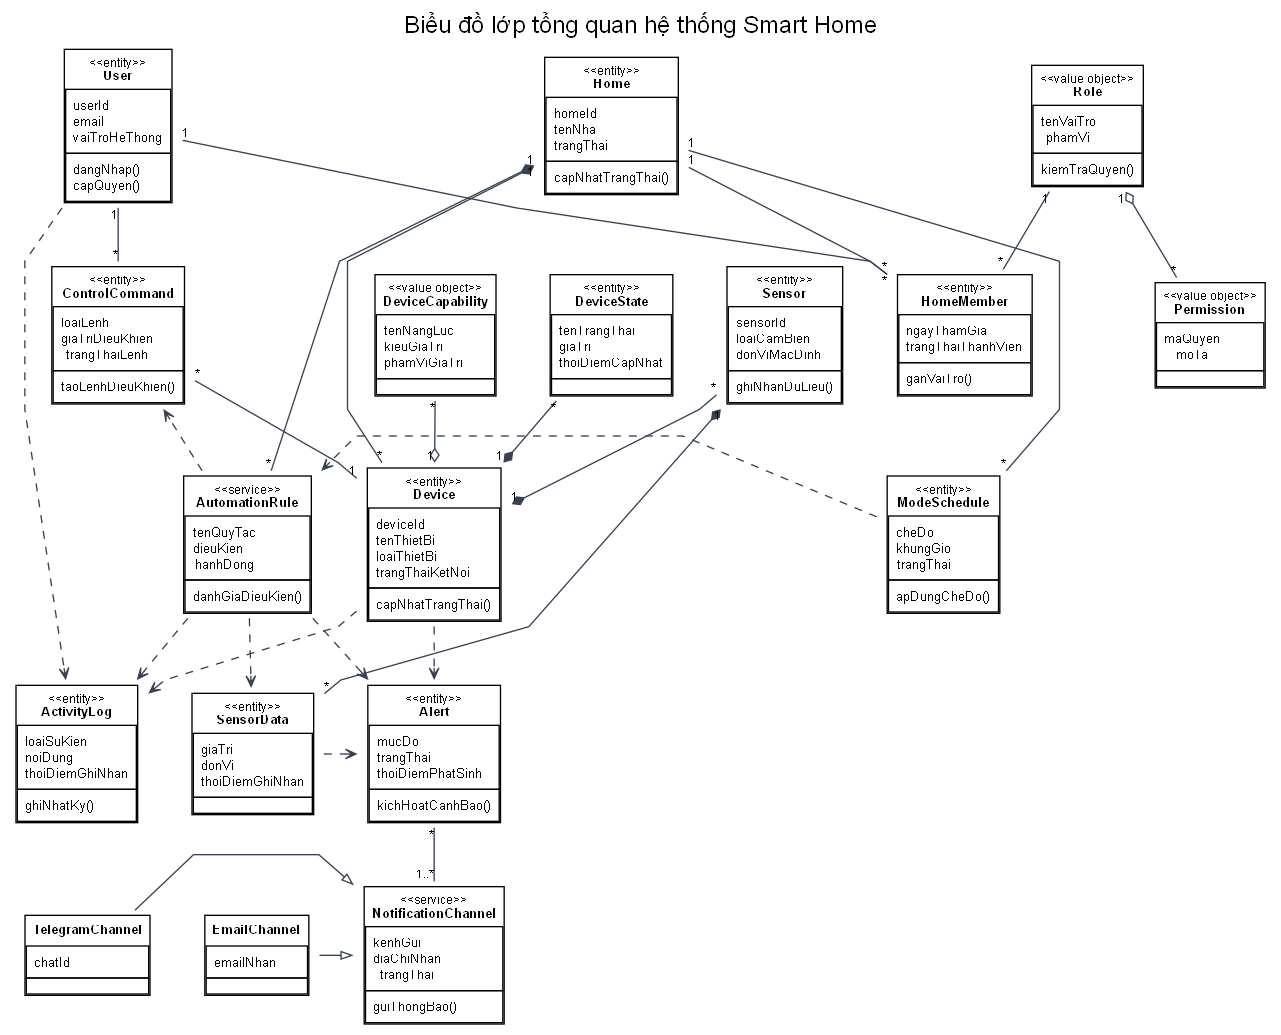
\includegraphics[width=\linewidth,height=0.78\textheight,keepaspectratio]{Images/class_system_overview.png}
    \caption{Biểu đồ lớp tổng quan hệ thống Smart Home}
    \label{fig:class-system-overview}
\end{figure}

Biểu đồ lớp mô tả các thực thể nghiệp vụ chính và quan hệ giữa chúng trong phạm vi hệ thống. Người dùng tham gia vào một hoặc nhiều Home thông qua HomeMember và Role. Home bao gồm các thiết bị, cảm biến, lịch chế độ và quy tắc tự động hóa. Dữ liệu cảm biến, trạng thái thiết bị, lệnh điều khiển, cảnh báo và nhật ký hoạt động tạo thành chuỗi thông tin phục vụ giám sát, điều khiển và truy vết trong hệ thống.

\textbf{Sequence diagram cho luồng gửi telemetry:}
\begin{figure}[htbp]
    \centering
    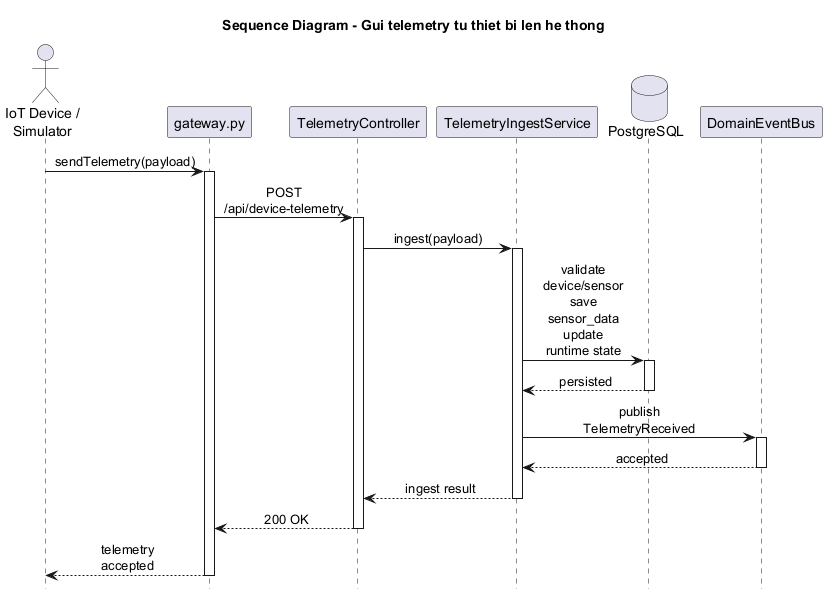
\includegraphics[width=\linewidth,height=0.72\textheight,keepaspectratio]{Images/sequence_telemetry_ingest.png}
    \caption{Sequence diagram cho luồng gửi telemetry}
    \label{fig:sequence-telemetry-ingest}
\end{figure}

Luồng gửi telemetry có actor thiết bị hoặc simulator, gateway, controller, service, database và event bus. Message chính đi từ \texttt{gateway.py} đến \texttt{TelemetryController}, sau đó \texttt{TelemetryIngestService} kiểm tra device/sensor, lưu \texttt{sensor\_data}, cập nhật runtime state và publish event nội bộ.

\textbf{Sequence diagram cho luồng thiết bị polling lệnh điều khiển:}
\begin{figure}[htbp]
    \centering
    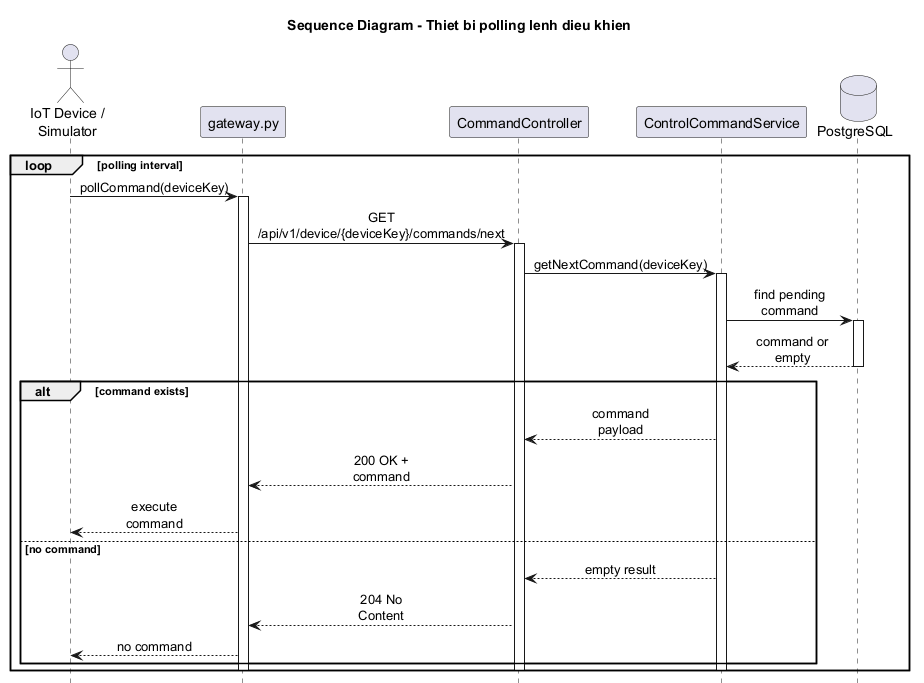
\includegraphics[width=\linewidth,height=0.72\textheight,keepaspectratio]{Images/sequence_command_polling.png}
    \caption{Sequence diagram cho luồng thiết bị polling lệnh điều khiển}
    \label{fig:sequence-command-polling}
\end{figure}

Luồng polling tách riêng vòng lặp lấy lệnh để hình không bị rối. \texttt{CommandController} gọi \texttt{ControlCommandService} để tìm command đang chờ trong PostgreSQL. Khung \texttt{alt} thể hiện hai nhánh: có lệnh thì trả payload để thiết bị thực thi, không có lệnh thì trả kết quả rỗng.

\textbf{Sequence diagram cho luồng ACK lệnh điều khiển:}
\begin{figure}[htbp]
    \centering
    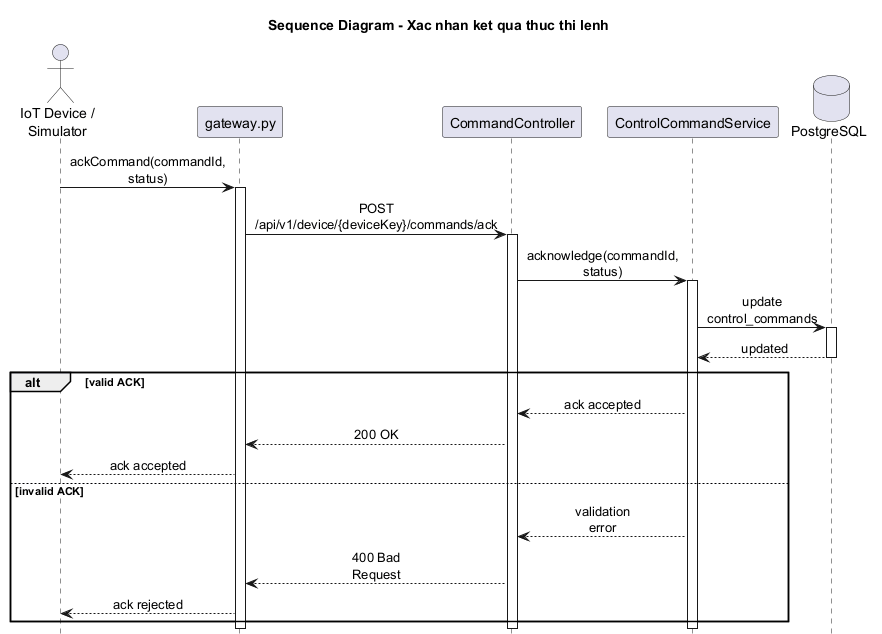
\includegraphics[width=\linewidth,height=0.72\textheight,keepaspectratio]{Images/sequence_command_ack.png}
    \caption{Sequence diagram cho luồng xác nhận kết quả thực thi lệnh}
    \label{fig:sequence-command-ack}
\end{figure}

Luồng ACK mô tả thiết bị gửi kết quả thực thi về gateway và backend. \texttt{ControlCommandService} cập nhật bảng \texttt{control\_commands}; khung \texttt{alt} thể hiện nhánh ACK hợp lệ và ACK không hợp lệ.

\textbf{Deployment diagram:}
\begin{figure}[htbp]
    \centering
    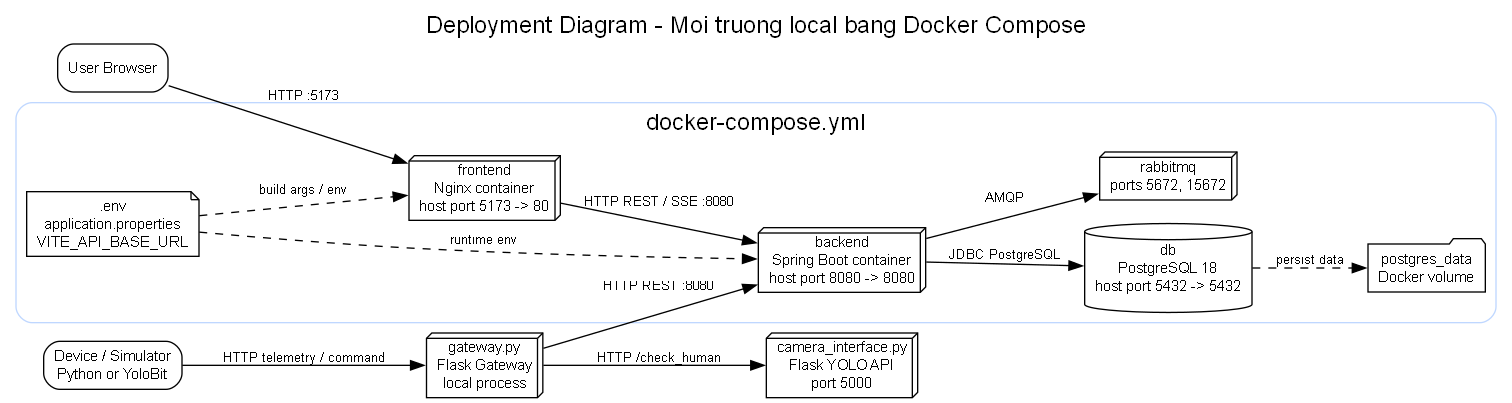
\includegraphics[width=\linewidth,height=0.78\textheight,keepaspectratio]{Images/deployment_local_docker.png}
    \caption{Deployment diagram cho môi trường chạy local bằng Docker Compose}
    \label{fig:deployment-local-docker}
\end{figure}

Deployment diagram phản ánh đúng \texttt{docker-compose.yml}: service \texttt{frontend} expose \texttt{5173:80}, service \texttt{backend} expose \texttt{8080:8080}, service \texttt{db} expose \texttt{5432:5432}, service \texttt{rabbitmq} expose \texttt{5672} và \texttt{15672}. Volume \texttt{postgres\_data} lưu dữ liệu PostgreSQL.

\subsection{Thiết kế ứng dụng}

\textbf{Thiết kế tầng giao diện:}
\begin{itemize}
    \item \texttt{frontend/src/router/AppRouter.jsx} định nghĩa các route chính: login, Google callback, dashboard, history, configs, settings, audit logs và trang lỗi.
    \item \texttt{frontend/src/pages} chứa màn hình nghiệp vụ; \texttt{frontend/src/components} chứa UI tái sử dụng như thẻ dashboard, bảng lịch, bảng audit, form cấu hình và layout.
    \item \texttt{AuthProvider.jsx}, \texttt{ProtectedRoute.jsx}, \texttt{RequireHomeRoute.jsx}, \texttt{RoleProtecteedRoute.jsx} kiểm soát phiên và quyền truy cập trên frontend.
\end{itemize}

\textbf{Thiết kế tầng xử lý nghiệp vụ:}
\begin{itemize}
    \item \texttt{controller} nhận request HTTP và chuyển yêu cầu sang service.
    \item \texttt{domain/service} điều phối use case như telemetry ingest, control command, config, dashboard, alert, audit, home user, schedule.
    \item \texttt{domain/provider} chứa strategy, policy và resolver cho xác thực, schedule, runtime state, device target và audit.
    \item \texttt{eventing} và \texttt{scheduler} xử lý event nội bộ, heartbeat dashboard, offline detection, manual hold, device schedule và outbox publisher.
\end{itemize}

\textbf{Thiết kế tầng dữ liệu:}
\begin{itemize}
    \item \texttt{persistence/entity} ánh xạ các bảng PostgreSQL như \texttt{users}, \texttt{homes}, \texttt{devices}, \texttt{sensors}, \texttt{sensor\_data}, \texttt{configs}, \texttt{control\_commands}, \texttt{alerts}, \texttt{activity\_logs}.
    \item \texttt{persistence/repo} chứa repository kế thừa \texttt{JpaRepository}.
    \item Migration chính nằm trong \texttt{backend/src/main/resources/db/migration/V1\_\_init.sql}; các migration sau bổ sung cột nguồn lệnh và index phục vụ realtime, audit, dashboard.
\end{itemize}

\textbf{Luồng request-response chính:}
\begin{itemize}
    \item \textbf{Đăng nhập:} \texttt{LoginPage} gọi \texttt{authApi.js}; backend nhận tại \texttt{AuthController}; service xác thực cấp token; frontend lưu phiên trong \texttt{authStorage.js}.
    \item \textbf{Dashboard realtime:} \texttt{DashboardPage} tải summary qua \texttt{DashboardController}; \texttt{dashboardRealtime.js} mở SSE để nhận cập nhật trạng thái.
    \item \textbf{Điều khiển thiết bị:} \texttt{DeviceSwitchCard} và hook dashboard gọi \texttt{/api/control/devices/\{deviceId\}}; backend đi qua \texttt{ControlController}, \texttt{ControlFacadeService}, \texttt{ManualControlService}, \texttt{DeviceCommandExecutionService}.
    \item \textbf{Telemetry:} thiết bị/gateway gọi \texttt{/api/device-telemetry}; backend lưu dữ liệu qua \texttt{TelemetryIngestService} và \texttt{TelemetryPersistenceService}.
    \item \textbf{Cấu hình tự động hóa:} \texttt{ConfigPage} gọi \texttt{ConfigController}; backend lưu \texttt{configs}, ghi audit và kích hoạt profile active.
\end{itemize}

\subsection{Cấu trúc thư mục và vai trò từng thành phần}

\begin{verbatim}
smart-house/
|-- backend/
|   |-- src/main/java/com/java/controller/
|   |-- src/main/java/com/java/domain/service/
|   |-- src/main/java/com/java/domain/provider/
|   |-- src/main/java/com/java/persistence/entity/
|   |-- src/main/java/com/java/persistence/repo/
|   |-- src/main/java/com/java/mapper/
|   |-- src/main/java/com/java/eventing/
|   |-- src/main/java/com/java/scheduler/
|   |-- src/main/resources/db/migration/
|   `-- src/test/java/
|-- frontend/
|   |-- src/pages/
|   |-- src/components/
|   |-- src/api/
|   |-- src/providers/
|   |-- src/router/
|   |-- src/hooks/
|   `-- src/utils/
|-- docs/
|   `-- diagram/
|-- Images/
|-- scripts/
|-- gateway.py
|-- camera_interface.py
|-- virtual_device_simulator.py
|-- aiot_code_v3.py
|-- docker-compose.yml
`-- main.tex, hcmut.sty, Sections/
\end{verbatim}

{\scriptsize
\setlength{\tabcolsep}{3pt}
\renewcommand{\arraystretch}{1.12}
\begin{longtable}{|p{0.19\textwidth}|p{0.27\textwidth}|p{0.28\textwidth}|p{0.17\textwidth}|}
\caption{Cấu trúc thư mục và vai trò từng thành phần}\\
\hline
\textbf{Thư mục / file} & \textbf{Loại nội dung} & \textbf{Vai trò trong hệ thống} & \textbf{Runtime / build / tài liệu} \\
\hline
\endfirsthead
\hline
\textbf{Thư mục / file} & \textbf{Loại nội dung} & \textbf{Vai trò trong hệ thống} & \textbf{Runtime / build / tài liệu} \\
\hline
\endhead
\texttt{backend/} & Spring Boot project, Maven, Dockerfile & Backend API, nghiệp vụ, persistence, migration, test & Runtime và build \\
\hline
\path{backend/src/main/java/com/java/controller} & REST controller & Endpoint cho auth, dashboard, telemetry, control, config, alert, audit, schedule & Runtime \\
\hline
\path{backend/src/main/java/com/java/domain/service} & Service nghiệp vụ & Điều phối use case và xử lý logic chính & Runtime \\
\hline
\path{backend/src/main/java/com/java/domain/provider} & Strategy, policy, resolver & Tách quy tắc nghiệp vụ và lựa chọn chiến lược & Runtime \\
\hline
\path{backend/src/main/java/com/java/persistence} & Entity và repository & Ánh xạ JPA và truy cập database & Runtime \\
\hline
\path{backend/src/main/resources/db/migration} & Flyway SQL migration & Khởi tạo schema, seed data, index và ràng buộc & Runtime khi ứng dụng khởi động \\
\hline
\texttt{frontend/} & React/Vite project, Dockerfile, Nginx config & Giao diện web và bản build static & Runtime frontend và build \\
\hline
\texttt{frontend/src/pages} & Route-level screens & Dashboard, History, Config, Settings, Audit, Auth & Runtime frontend \\
\hline
\texttt{frontend/src/components} & UI component & Card, table, modal, layout, form và filter & Runtime frontend \\
\hline
\texttt{frontend/src/api} & API client và service & Gọi backend, gắn token, refresh token, chuẩn hóa lỗi & Runtime frontend \\
\hline
\texttt{frontend/src/providers} & React Context provider & Quản lý trạng thái xác thực & Runtime frontend \\
\hline
\texttt{docs/diagram} & Sơ đồ tài liệu & Tài liệu kiến trúc, activity, sequence, state và sơ đồ sinh mới & Documentation \\
\hline
\texttt{Images/} & Hình report & Logo, use case, ERD, mapping, sơ đồ Graphviz sinh mới & Documentation \\
\hline
\texttt{gateway.py} & Flask gateway & Proxy telemetry, command, ack, YOLO và cache cục bộ cho thiết bị & Runtime hỗ trợ thiết bị \\
\hline
\texttt{camera\_interface.py} & Flask + OpenCV + YOLO & API nhận diện người/chuyển động qua camera & Runtime tùy chọn \\
\hline
\texttt{virtual\_device}\newline\texttt{\_simulator.py} & Python simulator & Mô phỏng telemetry, command, IR và trạng thái thiết bị & Runtime demo \\
\hline
\texttt{aiot\_code\_v3.py} & MicroPython/YoloBit & Mã thiết bị đọc cảm biến, điều khiển phần cứng và giao tiếp gateway & Runtime thiết bị \\
\hline
\texttt{scripts/} & Test script hỗ trợ & Kiểm thử gateway và cache camera & Test/support \\
\hline
\texttt{Sections/}, \texttt{main.tex} & LaTeX report & Nội dung báo cáo kỹ thuật & Documentation \\
\hline
\end{longtable}
}

\subsection{Design pattern được sử dụng}

{\scriptsize
\setlength{\tabcolsep}{3pt}
\renewcommand{\arraystretch}{1.12}
\begin{longtable}{|p{0.17\textwidth}|p{0.29\textwidth}|p{0.28\textwidth}|p{0.18\textwidth}|}
\caption{Design pattern được sử dụng trong hệ thống}\\
\hline
\textbf{Pattern} & \textbf{Vị trí hiện thực hóa} & \textbf{Cách xuất hiện trong ứng dụng} & \textbf{Lợi ích} \\
\hline
\endfirsthead
\hline
\textbf{Pattern} & \textbf{Vị trí hiện thực hóa} & \textbf{Cách xuất hiện trong ứng dụng} & \textbf{Lợi ích} \\
\hline
\endhead
Layered Architecture & \texttt{controller}, \texttt{domain/service}, \texttt{persistence/repo}, \texttt{persistence/entity}, \texttt{mapper} & Backend chia tầng HTTP, nghiệp vụ, ánh xạ dữ liệu và lưu trữ & Dễ bảo trì, giảm coupling, thuận lợi kiểm thử \\
\hline
MVC / REST Controller & \texttt{controller package} & Controller nhận request, service xử lý, entity/repository là model lưu trữ & Tách giao tiếp HTTP khỏi nghiệp vụ \\
\hline
Service Layer & \texttt{TelemetryIngestService}, \texttt{ControlFacadeService}, \texttt{ConfigService}, \texttt{DashboardService} & Service điều phối use case và transaction & Tập trung logic nghiệp vụ trong một tầng rõ ràng \\
\hline
Repository Pattern & \texttt{DeviceRepository}, \texttt{ConfigRepository}, \texttt{SensorDataRepository}, \texttt{ControlCommandRepository} & Repository kế thừa \texttt{JpaRepository} để truy cập dữ liệu & Che giấu chi tiết truy vấn và ORM khỏi service \\
\hline
Dependency Injection & Các class dùng \texttt{@Service}, \texttt{@Component}, \texttt{@RequiredArgsConstructor} & Spring tiêm dependency qua constructor & Dễ thay implementation và viết test \\
\hline
Strategy Pattern & \texttt{AuthenticationStrategy}, \texttt{ThresholdRuleStrategy}, \texttt{ScheduleExecutionStrategy} & Nhiều implementation cùng hợp đồng, resolver chọn strategy phù hợp & Mở rộng hành vi mà không làm phình service chính \\
\hline
Adapter Pattern & \texttt{DeviceCommandAdapter}, \texttt{MockOhstemDeviceAdapter} & Adapter tách nghiệp vụ điều khiển khỏi chi tiết thiết bị & Dễ thay đổi cách giao tiếp thiết bị \\
\hline
Factory Pattern & \texttt{ControlCommandFactory}, \texttt{DeviceEntityFactory}, \texttt{DeviceRuntimeStateFactory} & Gom quy tắc tạo entity và giá trị mặc định & Giảm lặp logic khởi tạo \\
\hline
Observer-style Eventing & \texttt{DomainEventBus}, \texttt{DomainEventListener}, \texttt{SimpleDomainEventBus} & Service publish event, listener xử lý realtime/audit/alert sau transaction & Giảm phụ thuộc trực tiếp giữa các module \\
\hline
DTO / Mapper Pattern & \texttt{controller/dto}, \texttt{mapper} & Request/response tách khỏi entity database & API ổn định và hạn chế lộ cấu trúc lưu trữ \\
\hline
Route Guard Pattern & \texttt{ProtectedRoute.jsx}, \texttt{RequireHomeRoute.jsx}, \texttt{RoleProtecteedRoute.jsx} & Frontend bảo vệ route theo trạng thái đăng nhập và role & Kiểm soát truy cập ở tầng giao diện \\
\hline
Provider Pattern & \texttt{AuthProvider.jsx} & React Context cung cấp auth state cho toàn ứng dụng & Tránh truyền props qua nhiều tầng \\
\hline
\end{longtable}
}

\subsection{Công nghệ sử dụng và lợi ích}

{\scriptsize
\setlength{\tabcolsep}{3pt}
\renewcommand{\arraystretch}{1.12}
\begin{longtable}{|p{0.17\textwidth}|p{0.28\textwidth}|p{0.24\textwidth}|p{0.23\textwidth}|}
\caption{Công nghệ sử dụng và lợi ích trong hệ thống}\\
\hline
\textbf{Công nghệ} & \textbf{Vị trí hiện thực hóa} & \textbf{Dùng ở đâu} & \textbf{Lợi ích trong hệ thống} \\
\hline
\endfirsthead
\hline
\textbf{Công nghệ} & \textbf{Vị trí hiện thực hóa} & \textbf{Dùng ở đâu} & \textbf{Lợi ích trong hệ thống} \\
\hline
\endhead
Java / Spring Boot & \texttt{backend/pom.xml}, \texttt{SmartHouseApplication.java} & Backend API và service & Nền tảng ổn định cho REST API, DI, validation, scheduler \\
\hline
Spring Web MVC & \texttt{spring-boot-starter-webmvc} & Controller HTTP, SSE & Triển khai endpoint và realtime stream \\
\hline
Spring Data JPA/JDBC & \texttt{spring-boot-starter-data-jpa}, \texttt{spring-boot-starter-data-jdbc} & Repository và entity & Truy cập PostgreSQL theo ORM/repository \\
\hline
Spring Security + JJWT & \texttt{SecurityConfig.java}, \texttt{JwtService.java}, \texttt{pom.xml} & JWT, route protection, password encoder & Xác thực stateless và phân quyền API \\
\hline
Flyway & \texttt{spring-boot-starter-flyway}, \texttt{db/migration} & Migration database & Quản lý schema và seed nhất quán \\
\hline
PostgreSQL & \texttt{docker-compose.yml}, \texttt{application.properties} & Database chính & Lưu dữ liệu quan hệ, ràng buộc, index, JSONB audit \\
\hline
RabbitMQ / Spring AMQP & \texttt{RabbitMqConfig.java}, \texttt{docker-compose.yml} & Outbox event và notification queue & Tách phát thông điệp khỏi transaction database \\
\hline
React & \texttt{frontend/package.json} & Frontend UI & Xây dựng giao diện component-based \\
\hline
Vite & \texttt{frontend/package.json}, \texttt{vite.config.js} & Dev/build frontend & Build nhanh và cấu hình gọn \\
\hline
React Router & \texttt{frontend/package.json}, \texttt{AppRouter.jsx} & Routing và route guard & Điều hướng màn hình và bảo vệ quyền truy cập \\
\hline
Recharts & \texttt{frontend/package.json}, \texttt{HistoryChartCard.jsx} & Biểu đồ lịch sử & Hiển thị dữ liệu sensor theo thời gian \\
\hline
Python Flask & \texttt{gateway.py}, \texttt{camera\_interface.py} & Gateway thiết bị và YOLO API & Tạo API nhẹ cho integration thiết bị \\
\hline
OpenCV / Ultralytics YOLO & \texttt{camera\_interface.py}, \texttt{yolov8n.pt}, \texttt{yolov8m.pt} & Nhận diện người/chuyển động & Bổ sung dữ liệu camera cho kịch bản an ninh \\
\hline
Docker Compose / Nginx & \texttt{docker-compose.yml}, \texttt{frontend/Dockerfile}, \texttt{frontend/nginx.conf} & Chạy frontend/backend/db/rabbitmq local & Đồng bộ môi trường demo và triển khai local \\
\hline
\end{longtable}
}

\subsection{Hướng dẫn cài đặt, cấu hình và sử dụng}

\textbf{Yêu cầu môi trường:}
\begin{itemize}
    \item Java JDK dùng để chạy backend. \texttt{pom.xml} khai báo \texttt{java.version=17}; Dockerfile backend dùng image build/run nền Java 21.
    \item Node.js và npm để cài dependency frontend; Dockerfile frontend dùng \texttt{node:20-alpine}.
    \item PostgreSQL cho database; Docker Compose dùng \texttt{postgres:18-alpine}.
    \item RabbitMQ cho message queue; Docker Compose dùng \texttt{rabbitmq:4.0-management}.
    \item Python để chạy \texttt{gateway.py}, \texttt{camera\_interface.py} và \texttt{virtual\_device\_simulator.py}.
    \item Docker và Docker Compose khi chạy toàn bộ stack bằng container.
\end{itemize}

\textbf{Cấu hình chính:}
\begin{itemize}
    \item Root project có file \texttt{.env} được \texttt{docker-compose.yml} sử dụng cho database, backend, RabbitMQ, mail, Telegram và Google OAuth.
    \item Backend đọc cấu hình trong \texttt{backend/src/main/resources/application.properties}, gồm \texttt{server.port=8080}, \texttt{DB\_URL}, \texttt{FLYWAY\_ENABLED}, JWT, RabbitMQ, mail và Telegram.
    \item Frontend nhận \texttt{VITE\_API\_BASE\_URL}, \texttt{VITE\_GOOGLE\_CLIENT\_ID}, \texttt{VITE\_GOOGLE\_REDIRECT\_URI} qua Docker build args hoặc môi trường Vite.
\end{itemize}

\textbf{Cài đặt và chạy thủ công:}
\begin{itemize}
    \item Backend: vào thư mục \texttt{backend}, chạy \texttt{.\\mvnw.cmd test} để kiểm thử hoặc \texttt{.\\mvnw.cmd spring-boot:run} để chạy server.
    \item Frontend: vào thư mục \texttt{frontend}, chạy \texttt{npm install}, sau đó \texttt{npm run dev}.
    \item Database: tạo database PostgreSQL trùng với cấu hình \texttt{DB\_URL}; Flyway tự chạy migration khi backend khởi động nếu \texttt{FLYWAY\_ENABLED=true}.
    \item Gateway thiết bị: chạy \texttt{python gateway.py} sau khi cấu hình biến môi trường liên quan đến backend và token thiết bị.
    \item Simulator: chạy \texttt{python virtual\_device\_simulator.py} để mô phỏng telemetry và command.
    \item Camera API: chạy \texttt{python camera\_interface.py}; service cung cấp \texttt{/health} và \texttt{/check\_human}.
\end{itemize}

\textbf{Chạy bằng Docker Compose:}
\begin{itemize}
    \item Từ root project, chạy \texttt{docker-compose up -d --build}.
    \item Frontend truy cập tại \texttt{http://localhost:5173}.
    \item Backend chạy tại \texttt{http://localhost:8080}.
    \item PostgreSQL expose tại \texttt{localhost:5432}.
    \item RabbitMQ expose AMQP tại \texttt{localhost:5672} và management UI tại \texttt{localhost:15672}.
\end{itemize}

\textbf{Khởi tạo dữ liệu:}
\begin{itemize}
    \item Flyway migration \texttt{V1\_\_init.sql} tạo schema, enum, trigger, index và dữ liệu seed.
    \item Các migration \texttt{V2} đến \texttt{V5} bổ sung cột \texttt{source} cho command và index phục vụ realtime/audit/dashboard.
    \item File \texttt{backend/db/init.sql} là script SQL khởi tạo khác đang có trong project.
\end{itemize}

\subsection{Kịch bản demo thực tế theo nghiệp vụ}

\textbf{Kịch bản 1: Giám sát môi trường phòng khách và phản ứng theo tình huống nóng}
\begin{itemize}
    \item \textbf{Bối cảnh:} Phòng khách có sensor nhiệt độ, độ ẩm, ánh sáng, chuyển động; quạt và đèn được điều khiển qua dashboard.
    \item \textbf{Vai trò người dùng:} Chủ nhà hoặc thành viên có quyền truy cập home.
    \item \textbf{Dữ liệu đầu vào:} Telemetry từ \texttt{virtual\_device\_simulator.py} hoặc \texttt{aiot\_code\_v3.py}.
    \item \textbf{Các bước thao tác:} Đăng nhập, mở Dashboard, quan sát monitoring card, đổi mode, điều chỉnh quạt/đèn dựa trên dữ liệu, mở History để đối chiếu dữ liệu thời gian.
    \item \textbf{Kết quả mong đợi:} Dashboard hiển thị dữ liệu realtime; \texttt{sensor\_data}, \texttt{device\_runtime\_state}, \texttt{device\_state\_history} được cập nhật.
    \item \textbf{Thành phần kỹ thuật:} \texttt{DashboardPage.jsx}, \texttt{dashboardApi.js}, \texttt{DashboardController.java}, \texttt{TelemetryIngestService.java}, \texttt{TelemetryPersistenceService.java}.
\end{itemize}

\textbf{Kịch bản 2: Cấu hình tự động hóa theo ngưỡng nhiệt độ và ánh sáng}
\begin{itemize}
    \item \textbf{Bối cảnh:} Chủ nhà muốn quạt tự phản ứng với nhiệt độ và đèn tự phản ứng với ánh sáng.
    \item \textbf{Vai trò người dùng:} Owner, co-owner hoặc admin.
    \item \textbf{Dữ liệu đầu vào:} Ngưỡng \texttt{thigh}, \texttt{tlow}, \texttt{lhigh}, \texttt{llow}, \texttt{tcritical}; thiết bị giám sát và thiết bị đích.
    \item \textbf{Các bước thao tác:} Mở Config, chỉnh threshold, gán sensor/actuator, lưu cấu hình, kích hoạt profile, quan sát audit log.
    \item \textbf{Kết quả mong đợi:} Bảng \texttt{configs} cập nhật; khi telemetry phù hợp đến, \texttt{ModeAutomationService} áp dụng policy cho quạt hoặc đèn.
    \item \textbf{Thành phần kỹ thuật:} \texttt{ConfigPage.jsx}, \texttt{configApi.js}, \texttt{ConfigController.java}, \texttt{ConfigService.java}, \texttt{FanAutomationPolicy.java}, \texttt{LightAutomationPolicy.java}.
\end{itemize}

\textbf{Kịch bản 3: Truy vết cảnh báo và hoạt động hệ thống}
\begin{itemize}
    \item \textbf{Bối cảnh:} Hệ thống phát sinh cảnh báo do sensor, thiết bị offline hoặc thao tác điều khiển.
    \item \textbf{Vai trò người dùng:} Admin hoặc người có quyền xem audit.
    \item \textbf{Dữ liệu đầu vào:} Alert, activity log, thay đổi cấu hình và sự kiện thiết bị.
    \item \textbf{Các bước thao tác:} Mở Audit Logs, lọc theo nhóm sự kiện, tìm kiếm từ khóa, xem thay đổi cấu hình và trạng thái cảnh báo.
    \item \textbf{Kết quả mong đợi:} Giao diện hiển thị dữ liệu từ \texttt{activity\_logs} và \texttt{alerts}; người dùng truy vết được thời điểm và nguồn thay đổi.
    \item \textbf{Thành phần kỹ thuật:} \texttt{AuditLogsPage.jsx}, \texttt{auditApi.js}, \texttt{AuditQueryController.java}, \texttt{ActivityLogRepository.java}, \texttt{AlertRepository.java}.
\end{itemize}

\textbf{Kịch bản 4: Quản lý lịch mode và quyền thành viên}
\begin{itemize}
    \item \textbf{Bối cảnh:} Home có nhiều thành viên và cần lịch chuyển mode theo khung giờ.
    \item \textbf{Vai trò người dùng:} Owner hoặc co-owner.
    \item \textbf{Dữ liệu đầu vào:} Lịch mode, vai trò thành viên, quyền kích hoạt profile.
    \item \textbf{Các bước thao tác:} Mở Settings, tạo/sửa mode schedule, cập nhật quyền thành viên, kiểm tra kết quả trên dashboard.
    \item \textbf{Kết quả mong đợi:} Lịch được lưu và scheduler thực thi; quyền thành viên cập nhật trong \texttt{home\_users}.
    \item \textbf{Thành phần kỹ thuật:} Settings page, ModeSchedule controller/service, HomeUser controller và HomeUserManagement service.
\end{itemize}

\subsection{Đối chiếu hiện thực hóa thiết kế}

Các bảng dưới đây đối chiếu các nhóm thiết kế với vị trí hiện thực hóa tương ứng trong dự án. Các đường dẫn backend được rút gọn từ prefix \path{backend/src/main/java/com/java/} để tránh làm vỡ cột khi trình bày.

{\scriptsize
\setlength{\tabcolsep}{3pt}
\renewcommand{\arraystretch}{1.14}
\begin{longtable}{|p{0.18\textwidth}|p{0.30\textwidth}|p{0.32\textwidth}|p{0.14\textwidth}|}
\caption{Đối chiếu hiện thực hóa nhóm cấu hình dự án và triển khai}\\
\hline
\textbf{Nhóm} & \textbf{File/thư mục} & \textbf{Vai trò} & \textbf{Mapping} \\
\hline
\endfirsthead
\hline
\textbf{Nhóm} & \textbf{File/thư mục} & \textbf{Vai trò} & \textbf{Mapping} \\
\hline
\endhead
Docker Compose & \path{docker-compose.yml} & Định nghĩa service \texttt{db}, \texttt{rabbitmq}, \texttt{backend}, \texttt{frontend}, port và volume. & Deployment \\
\hline
Backend build & \path{backend/pom.xml} & Khai báo Spring Boot, JPA, Security, Flyway, PostgreSQL, RabbitMQ, Mail và test dependency. & Công nghệ \\
\hline
Backend config & \path{backend/src/main/resources/application.properties} & Khai báo port, datasource, Flyway, JWT, RabbitMQ, Mail, Telegram và SSE config. & Cấu hình \\
\hline
Backend image & \path{backend/Dockerfile} & Build jar bằng Maven và chạy Spring Boot API tại cổng 8080. & Runtime \\
\hline
Frontend build & \path{frontend/package.json} & Khai báo React, React Router, Recharts, Axios, Vite và scripts frontend. & Công nghệ \\
\hline
Frontend image & \path{frontend/Dockerfile} & Build React/Vite app bằng Node và phục vụ static build. & Runtime \\
\hline
Frontend server & \path{frontend/nginx.conf} & Cấu hình Nginx phục vụ frontend trong container. & Deployment \\
\hline
\end{longtable}
}

{\scriptsize
\setlength{\tabcolsep}{3pt}
\renewcommand{\arraystretch}{1.14}
\begin{longtable}{|p{0.18\textwidth}|p{0.30\textwidth}|p{0.32\textwidth}|p{0.14\textwidth}|}
\caption{Đối chiếu hiện thực hóa nhóm giao diện web}\\
\hline
\textbf{Nhóm} & \textbf{File/thư mục} & \textbf{Vai trò} & \textbf{Mapping} \\
\hline
\endfirsthead
\hline
\textbf{Nhóm} & \textbf{File/thư mục} & \textbf{Vai trò} & \textbf{Mapping} \\
\hline
\endhead
Routing & \path{frontend/src/router/AppRouter.jsx} & Định nghĩa route, route guard và luồng điều hướng chính của ứng dụng. & UI layer \\
\hline
Auth state & \path{frontend/src/providers/AuthProvider.jsx} & Cung cấp trạng thái xác thực và thông tin người dùng cho frontend. & Provider \\
\hline
Auth storage & \path{frontend/src/utils/authStorage.js} & Lưu, đọc và xóa token/session ở phía frontend. & Auth \\
\hline
API client & \path{frontend/src/api/apiClient.js} & Gọi backend, gắn bearer token, refresh token và chuẩn hóa lỗi API. & Request \\
\hline
Auth API & \path{frontend/src/api/authApi.js} & Gửi request đăng nhập, refresh token và lấy thông tin phiên. & Auth \\
\hline
Dashboard API & \path{frontend/src/api/dashboardApi.js} & Tải dữ liệu dashboard và phục vụ realtime dashboard. & Dashboard \\
\hline
Config API & \path{frontend/src/api/configApi.js} & Gọi backend cho cấu hình tự động hóa và profile active. & Config \\
\hline
Dashboard page & \path{frontend/src/pages/dashboard/DashboardPage.jsx} & Màn hình giám sát trạng thái thiết bị và dữ liệu realtime. & Demo \\
\hline
Config page & \path{frontend/src/pages/config/ConfigPage.jsx} & Màn hình cấu hình ngưỡng và thiết bị giám sát. & Demo \\
\hline
History page & \path{frontend/src/pages/history/HistoryPage.jsx} & Hiển thị lịch sử sensor và biểu đồ dữ liệu. & History \\
\hline
Settings/Audit & \path{frontend/src/pages/settings}, \path{frontend/src/pages/audit} & Quản lý thành viên, lịch mode và nhật ký hoạt động. & Admin UI \\
\hline
UI components & \path{frontend/src/components} & Chứa card, table, modal, form, layout và filter dùng lại. & UI component \\
\hline
\end{longtable}
}

{\scriptsize
\setlength{\tabcolsep}{3pt}
\renewcommand{\arraystretch}{1.14}
\begin{longtable}{|p{0.18\textwidth}|p{0.30\textwidth}|p{0.32\textwidth}|p{0.14\textwidth}|}
\caption{Đối chiếu hiện thực hóa nhóm backend API}\\
\hline
\textbf{Nhóm} & \textbf{File/thư mục} & \textbf{Vai trò} & \textbf{Mapping} \\
\hline
\endfirsthead
\hline
\textbf{Nhóm} & \textbf{File/thư mục} & \textbf{Vai trò} & \textbf{Mapping} \\
\hline
\endhead
Backend entry & \path{SmartHouseApplication.java} & Entry point Spring Boot và bootstrap toàn bộ backend. & Runtime \\
\hline
Auth API & \path{controller/AuthController.java} & Nhận request đăng nhập, refresh token và thông tin phiên. & API layer \\
\hline
Dashboard API & \path{controller/DashboardController.java} & Cung cấp dashboard summary và stream SSE cho home. & Dashboard \\
\hline
Telemetry API & \path{controller/TelemetryController.java} & Nhận telemetry từ gateway hoặc thiết bị. & Telemetry \\
\hline
Control API & \path{controller/ControlController.java} & Nhận thao tác điều khiển từ frontend. & Control \\
\hline
Command API & \path{controller/CommandController.java} & Cung cấp polling command và ACK cho thiết bị. & Device API \\
\hline
Config API & \path{controller/ConfigController.java} & Quản lý cấu hình tự động hóa và profile active. & Config \\
\hline
Alert API & \path{controller/AlertController.java} & Truy vấn và cập nhật trạng thái cảnh báo. & Alert \\
\hline
Audit API & \path{controller/AuditQueryController.java} & Truy vấn nhật ký hoạt động và bộ lọc audit. & Audit \\
\hline
Device/User/Schedule API & \path{controller/DeviceController.java}, \path{HomeUserController.java}, \path{ModeScheduleController.java} & Quản lý thiết bị, thành viên home và lịch mode. & Management \\
\hline
Security config & \path{config/SecurityConfig.java} & Cấu hình JWT filter, CORS, public endpoint và password encoder. & Security \\
\hline
Exception handler & \path{GlobalExceptionHandler.java} & Chuẩn hóa response lỗi validation, not found, forbidden và lỗi hệ thống. & Error handling \\
\hline
\end{longtable}
}

{\scriptsize
\setlength{\tabcolsep}{3pt}
\renewcommand{\arraystretch}{1.14}
\begin{longtable}{|p{0.18\textwidth}|p{0.30\textwidth}|p{0.32\textwidth}|p{0.14\textwidth}|}
\caption{Đối chiếu hiện thực hóa nhóm xử lý nghiệp vụ, sự kiện và lịch}\\
\hline
\textbf{Nhóm} & \textbf{File/thư mục} & \textbf{Vai trò} & \textbf{Mapping} \\
\hline
\endfirsthead
\hline
\textbf{Nhóm} & \textbf{File/thư mục} & \textbf{Vai trò} & \textbf{Mapping} \\
\hline
\endhead
Telemetry service & \path{domain/service/TelemetryIngestService.java} & Điều phối luồng nhận telemetry và kích hoạt xử lý sau lưu. & Service \\
\hline
Telemetry persistence & \path{domain/service/TelemetryPersistenceService.java} & Kiểm tra device/sensor, lưu \texttt{sensor\_data}, cập nhật runtime state. & Database \\
\hline
Telemetry automation & \path{domain/service/TelemetryAutomationService.java} & Kích hoạt tự động hóa khi telemetry thuộc cấu hình active. & Automation \\
\hline
Control facade & \path{domain/service/ControlFacadeService.java} & Điều phối điều khiển manual và auto. & Facade \\
\hline
Command service & \path{domain/service/ControlCommandService.java} & Tạo, lấy, gửi và xác nhận command cho thiết bị. & Command \\
\hline
Config/Dashboard & \path{domain/service/ConfigService.java}, \path{DashboardService.java} & Xử lý cấu hình tự động hóa và dữ liệu dashboard. & Use case \\
\hline
Alert/Audit & \path{domain/service/AlertService.java}, \path{ActivityLogService.java} & Xử lý cảnh báo và nhật ký hoạt động. & Monitoring \\
\hline
Auth strategy & \path{domain/provider/AuthenticationStrategy.java} & Định nghĩa hợp đồng strategy xác thực. & Pattern \\
\hline
Auth providers & \path{domain/provider/LocalAuthenticationStrategy.java}, \path{GoogleAuthenticationStrategy.java} & Triển khai xác thực local và Google. & Pattern \\
\hline
Threshold strategy & \path{domain/service/ThresholdRuleStrategy.java} & Định nghĩa hợp đồng kiểm tra ngưỡng sensor. & Pattern \\
\hline
Threshold implementations & \path{TemperatureThresholdStrategy.java}, \path{LightThresholdStrategy.java}, \path{HumidityThresholdStrategy.java}, \path{MotionThresholdStrategy.java} & Kiểm tra ngưỡng nhiệt độ, ánh sáng, độ ẩm và chuyển động. & Alert \\
\hline
Event bus & \path{eventing/DomainEventBus.java}, \path{SimpleDomainEventBus.java} & Publish và dispatch domain event nội bộ. & Observer \\
\hline
Realtime listeners & \path{eventing/DashboardRealtimeTelemetryListener.java}, \path{CommandLongPollListener.java} & Phát dashboard realtime và long-poll command. & Realtime \\
\hline
Schedulers & \path{scheduler/OfflineScheduler.java}, \path{DeviceScheduleScheduler.java}, \path{ManualHoldScheduler.java}, \path{ModeAutomationScheduler.java} & Job nền cho offline, schedule, manual hold và mode automation. & Scheduler \\
\hline
\end{longtable}
}

{\scriptsize
\setlength{\tabcolsep}{3pt}
\renewcommand{\arraystretch}{1.14}
\begin{longtable}{|p{0.18\textwidth}|p{0.30\textwidth}|p{0.32\textwidth}|p{0.14\textwidth}|}
\caption{Đối chiếu hiện thực hóa nhóm lưu trữ dữ liệu}\\
\hline
\textbf{Nhóm} & \textbf{File/thư mục} & \textbf{Vai trò} & \textbf{Mapping} \\
\hline
\endfirsthead
\hline
\textbf{Nhóm} & \textbf{File/thư mục} & \textbf{Vai trò} & \textbf{Mapping} \\
\hline
\endhead
Migration chính & \path{backend/src/main/resources/db/migration/V1__init.sql} & Tạo enum, bảng, trigger, constraint, index và seed data. & Schema \\
\hline
Migration bổ sung & \path{V2__add_control_command_source.sql} đến \path{V5__audit_dashboard_pagination_indexes.sql} & Bổ sung cột source và index phục vụ command, audit, dashboard. & Schema \\
\hline
Device repository & \path{persistence/repo/DeviceRepository.java} & Truy vấn thiết bị, trạng thái và phạm vi home. & Repository \\
\hline
Sensor repository & \path{persistence/repo/SensorRepository.java}, \path{SensorDataRepository.java} & Truy vấn sensor và dữ liệu telemetry. & Repository \\
\hline
Config repository & \path{persistence/repo/ConfigRepository.java} & Truy vấn cấu hình và profile active. & Repository \\
\hline
Command repository & \path{persistence/repo/ControlCommandRepository.java} & Truy vấn command pending, sent, acked. & Repository \\
\hline
Audit repository & \path{persistence/repo/ActivityLogRepository.java}, \path{AlertRepository.java} & Truy vấn activity log và alert. & Repository \\
\hline
User/Home repository & \path{persistence/repo/UserRepository.java}, \path{HomeRepository.java}, \path{HomeUserRepository.java} & Truy vấn user, home và membership. & Repository \\
\hline
Outbox repository & \path{persistence/repo/OutboxEventRepository.java} & Lưu sự kiện tích hợp cần publish qua RabbitMQ. & Integration \\
\hline
Device entities & \path{persistence/entity/DeviceEntity.java}, \path{DeviceCapabilityEntity.java}, \path{DeviceRuntimeStateEntity.java} & Ánh xạ bảng thiết bị, capability và trạng thái runtime. & Entity \\
\hline
Sensor entities & \path{persistence/entity/SensorEntity.java}, \path{SensorDataEntity.java} & Ánh xạ sensor và dữ liệu telemetry. & Entity \\
\hline
Control entities & \path{persistence/entity/ConfigEntity.java}, \path{ControlCommandEntity.java}, \path{ScheduleEntity.java} & Ánh xạ cấu hình, command và lịch. & Entity \\
\hline
Identity entities & \path{persistence/entity/UserEntity.java}, \path{HomeEntity.java}, \path{HomeUserEntity.java} & Ánh xạ người dùng, nhà và thành viên. & Entity \\
\hline
Monitoring entities & \path{persistence/entity/AlertEntity.java}, \path{ActivityLogEntity.java}, \path{OutboxEventEntity.java} & Ánh xạ cảnh báo, audit và outbox event. & Entity \\
\hline
\end{longtable}
}

{\scriptsize
\setlength{\tabcolsep}{3pt}
\renewcommand{\arraystretch}{1.14}
\begin{longtable}{|p{0.18\textwidth}|p{0.30\textwidth}|p{0.32\textwidth}|p{0.14\textwidth}|}
\caption{Đối chiếu hiện thực hóa nhóm gateway, thiết bị, mô phỏng và camera}\\
\hline
\textbf{Nhóm} & \textbf{File/thư mục} & \textbf{Vai trò} & \textbf{Mapping} \\
\hline
\endfirsthead
\hline
\textbf{Nhóm} & \textbf{File/thư mục} & \textbf{Vai trò} & \textbf{Mapping} \\
\hline
\endhead
Gateway & \path{gateway.py} & Flask gateway chuyển telemetry, command, ACK và camera proxy. & Integration \\
\hline
Simulator & \path{virtual_device_simulator.py} & Mô phỏng sensor, command, IR, cửa, quạt và đèn. & Demo \\
\hline
Firmware & \path{aiot_code_v3.py} & Mã YoloBit/OhStem đọc sensor, LCD, IR, command và telemetry. & Device \\
\hline
Camera API & \path{camera_interface.py} & Flask API dùng OpenCV/YOLO cho nhận diện người/chuyển động. & Camera \\
\hline
YOLO model & \path{yolov8n.pt}, \path{yolov8m.pt} & Model nhận diện được camera service sử dụng khi chạy. & Asset \\
\hline
\end{longtable}
}

{\scriptsize
\setlength{\tabcolsep}{3pt}
\renewcommand{\arraystretch}{1.14}
\begin{longtable}{|p{0.18\textwidth}|p{0.30\textwidth}|p{0.32\textwidth}|p{0.14\textwidth}|}
\caption{Đối chiếu hiện thực hóa nhóm tài liệu, kiểm thử và tài nguyên}\\
\hline
\textbf{Nhóm} & \textbf{File/thư mục} & \textbf{Vai trò} & \textbf{Mapping} \\
\hline
\endfirsthead
\hline
\textbf{Nhóm} & \textbf{File/thư mục} & \textbf{Vai trò} & \textbf{Mapping} \\
\hline
\endhead
README & \path{Readme.md} & Tài liệu hướng dẫn tổng quan project. & Documentation \\
\hline
API docs & \path{docs/api-design-patterns.md} & Ghi chú API và pattern hỗ trợ đối chiếu thiết kế. & Documentation \\
\hline
Schema docs & \path{docs/smart_home_schema_documentation.md} & Tài liệu mô tả schema smart home. & Database \\
\hline
Generated diagrams & \path{docs/diagram/report_generated} & Chứa source sơ đồ sinh mới cho report. & Diagram \\
\hline
Report images & \path{Images/} & Chứa logo, use case, ERD, mapping và ảnh sơ đồ. & Asset \\
\hline
Backend tests & \path{backend/src/test/java} & Unit/integration test cho backend. & Test \\
\hline
Gateway tests & \path{scripts/test_gateway_ack_queue.py} & Kiểm thử hàng đợi ACK gateway. & Test \\
\hline
Camera tests & \path{scripts/test_camera_check_human_cached.py} & Kiểm thử cache API nhận diện người. & Test \\
\hline
\end{longtable}
}
